% ******************************* PhD Thesis Template **************************
% Please have a look at the README.md file for info on how to use the template

\documentclass[a4paper,12pt,times,twoside,print, draft]{Classes/PhDThesisPSnPDF}

% ******************************************************************************
% ******************************* Class Options ********************************
% *********************** See README for more details **************************
% ******************************************************************************

% `a4paper'(The University of Cambridge PhD thesis guidelines recommends a page
% size a4 - default option) or `a5paper': A5 Paper size is also allowed as per
% the Cambridge University Engineering Deparment guidelines for PhD thesis
%
% `11pt' or `12pt'(default): Font Size 10pt is NOT recommended by the University
% guidelines
%
% `oneside' or `twoside'(default): Printing double side (twoside) or single
% side.
%
% `print': Use `print' for print version with appropriate margins and page
% layout. Leaving the options field blank will activate Online version.
%
% `index': For index at the end of the thesis
%
% `draftclassic': For draft mode without loading any images (same as draft in book)
%
% `draft': Special draft mode with line numbers, images, and water mark with
% timestamp and custom text. Position of the text can also be modified.
%
% `abstract': To generate only the title page and abstract page with
% dissertation title and name, to submit to the Student Registry
%
% `chapter`: This option enables only the specified chapter and it's references
%  Useful for review and corrections.
%
% ************************* Custom Page Margins ********************************
%
% `custommargin`: Use `custommargin' in options to activate custom page margins,
% which can be defined in the preamble.tex. Custom margin will override
% print/online margin setup.
%
% *********************** Choosing the Fonts in Class Options ******************
%
% `times' : Times font with math support. (The Cambridge University guidelines
% recommend using times)
%
% `fourier': Utopia Font with Fourier Math font (Font has to be installed)
%            It's a free font.
%
% `customfont': Use `customfont' option in the document class and load the
% package in the preamble.tex
%
% default or leave empty: `Latin Modern' font will be loaded.
%
% ********************** Choosing the Bibliography style ***********************
%
% `authoryear': For author-year citation eg., Krishna (2013)
%
% `numbered': (Default Option) For numbered and sorted citation e.g., [1,5,2]
%
% `custombib': Define your own bibliography style in the `preamble.tex' file.
%              `\RequirePackage[square, sort, numbers, authoryear]{natbib}'.
%              This can be also used to load biblatex instead of natbib
%              (See Preamble)
%
% **************************** Choosing the Page Style *************************
%
% `default (leave empty)': For Page Numbers in Header (Left Even, Right Odd) and
% Chapter Name in Header (Right Even) and Section Name (Left Odd). Blank Footer.
%
% `PageStyleI': Chapter Name next & Page Number on Even Side (Left Even).
% Section Name & Page Number in Header on Odd Side (Right Odd). Footer is empty.
%
% `PageStyleII': Chapter Name on Even Side (Left Even) in Header. Section Number
% and Section Name in Header on Odd Side (Right Odd). Page numbering in footer

% Uncomment to change page style
%\pagestyle{PageStyleII}

% ********************************** Preamble **********************************
% Preamble: Contains packages and user-defined commands and settings
% ******************************************************************************
% ****************************** Custom Margin *********************************

% Add `custommargin' in the document class options to use this section
% Set {innerside margin / outerside margin / topmargin / bottom margin}  and
% other page dimensions
\ifsetCustomMargin
  \RequirePackage[left=37mm,right=30mm,top=35mm,bottom=30mm]{geometry}
  \setFancyHdr % To apply fancy header after geometry package is loaded
\fi

% Add spaces between paragraphs
%\setlength{\parskip}{0.5em}
% Ragged bottom avoids extra whitespaces between paragraphs
\raggedbottom
% To remove the excess top spacing for enumeration, list and description
%\usepackage{enumitem}
%\setlist[enumerate,itemize,description]{topsep=0em}

% *****************************************************************************
% ******************* Fonts (like different typewriter fonts etc.)*************

% Add `customfont' in the document class option to use this section

\ifsetCustomFont
  % Set your custom font here and use `customfont' in options. Leave empty to
  % load computer modern font (default LaTeX font).
  %\RequirePackage{helvet}

  % For use with XeLaTeX
  %  \setmainfont[
  %    Path              = ./libertine/opentype/,
  %    Extension         = .otf,
  %    UprightFont = LinLibertine_R,
  %    BoldFont = LinLibertine_RZ, % Linux Libertine O Regular Semibold
  %    ItalicFont = LinLibertine_RI,
  %    BoldItalicFont = LinLibertine_RZI, % Linux Libertine O Regular Semibold Italic
  %  ]
  %  {libertine}
  %  % load font from system font
  %  \newfontfamily\libertinesystemfont{Linux Libertine O}
\fi

% *****************************************************************************
% **************************** Custom Packages ********************************

% ***************************  Language ***********************************
\usepackage[ngerman]{babel}
\usepackage[utf8]{inputenc}
\declarationtitle{}
\abstracttitle{Abstract}
\acknowledgementstitle{Acknowledgements}


% ************************* Algorithms and Pseudocode **************************

%\usepackage{algpseudocode}


% ********************Captions and Hyperreferencing / URL **********************

% Captions: This makes captions of figures use a boldfaced small font.
%\RequirePackage[small,bf]{caption}

\RequirePackage[labelsep=space,tableposition=top]{caption}
\renewcommand{\figurename}{Fig.} %to support older versions of captions.sty


% *************************** Graphics and figures *****************************

%\usepackage{rotating}
%\usepackage{wrapfig}

% Uncomment the following two lines to force Latex to place the figure.
% Use [H] when including graphics. Note 'H' instead of 'h'
%\usepackage{float}
%\restylefloat{figure}

% Subcaption package is also available in the sty folder you can use that by
% uncommenting the following line
% This is for people stuck with older versions of texlive
%\usepackage{sty/caption/subcaption}
\usepackage{subcaption}

% ********************************** Tables ************************************
\usepackage{booktabs} % For professional looking tables
\usepackage{multirow}
\usepackage{makecell}

%\usepackage{multicol}
%\usepackage{longtable}
\usepackage{tabularx}
\usepackage{adjustbox}


% *********************************** SI Units *********************************
\usepackage{siunitx} % use this package module for SI units


% ******************************* Line Spacing *********************************

% Choose linespacing as appropriate. Default is one-half line spacing as per the
% University guidelines

% \doublespacing
% \onehalfspacing
% \singlespacing


% ************************ Formatting / Footnote *******************************

% Don't break enumeration (etc.) across pages in an ugly manner (default 10000)
%\clubpenalty=500
%\widowpenalty=500

%\usepackage[perpage]{footmisc} %Range of footnote options


% *****************************************************************************
% *************************** Bibliography  and References ********************

%\usepackage{cleveref} %Referencing without need to explicitly state fig /table

% Add `custombib' in the document class option to use this section
\ifuseCustomBib
  %   \RequirePackage[square, sort, numbers, authoryear]{natbib} % CustomBib

  % If you would like to use biblatex for your reference management, as opposed to the default `natbibpackage` pass the option `custombib` in the document class. Comment out the previous line to make sure you don't load the natbib package. Uncomment the following lines and specify the location of references.bib file

  \RequirePackage[backend=biber, style=numeric,citestyle=numeric, sorting=none,maxnames=2,maxbibnames=8,minbibnames=8]{biblatex} %  citestyle=numeric, sorting=nty, natbib=true
  \addbibresource{References/references.bib} %Location of references.bib only for biblatex, Do not omit the .bib extension from the filename.
  %\DeclareLanguageMapping{ngerman}{ngerman-apa}

\fi

% changes the default name `Bibliography` -> `References'
\renewcommand{\bibname}{Test}

% german und instead of and
%\usepackage{bibgerm}

\usepackage{url} % use url in bib
\usepackage{hyperref} % call this -> autoref works
%\usepackage[style=apa,backend=biber,isbn=false,maxnames=2,maxbibnames=8,minbibnames=8]{biblatex}



% ******************************************************************************
% ************************* User Defined Commands ******************************
% ******************************************************************************

% *********** To change the name of Table of Contents / LOF and LOT ************

%\renewcommand{\contentsname}{My Table of Contents}
%\renewcommand{\listfigurename}{My List of Figures}
%\renewcommand{\listtablename}{My List of Tables}


% ********************** TOC depth and numbering depth *************************

\setcounter{secnumdepth}{2}
\setcounter{tocdepth}{2}


% ******************************* Nomenclature *********************************

% To change the name of the Nomenclature section, uncomment the following line

%\renewcommand{\nomname}{Symbols}


% ********************************* Appendix ***********************************

% The default value of both \appendixtocname and \appendixpagename is `Appendices'. These names can all be changed via:

%\renewcommand{\appendixtocname}{List of appendices}
%\renewcommand{\appendixname}{Appndx}
\newcommand*{\Anhangautorefname}{Anhang}

% *********************** Configure Draft Mode **********************************

% Uncomment to disable figures in `draft'
%\setkeys{Gin}{draft=true}  % set draft to false to enable figures in `draft'

% These options are active only during the draft mode
% Default text is "Draft"
%\SetDraftText{DRAFT}

% Default Watermark location is top. Location (top/bottom)
%\SetDraftWMPosition{bottom}

% Draft Version - default is v1.0
%\SetDraftVersion{v1.1}

% Draft Text grayscale value (should be between 0-black and 1-white)
% Default value is 0.75
%\SetDraftGrayScale{0.8}


% ******************************** Todo Notes **********************************
%% Uncomment the following lines to have todonotes.

\ifsetDraft
  \usepackage[colorinlistoftodos]{todonotes}
  \newcommand{\mynote}[1]{\todo[author=lars,size=\small,inline,color=green!40]{#1}}
\else
  \newcommand{\mynote}[1]{}
  \newcommand{\listoftodos}{}
\fi

% Example todo: \mynote{Hey! I have a note}

% *****************************************************************************
% ******************* Better enumeration my MB*************
\usepackage{enumitem}

%************************** acronyms *******************
\usepackage[printonlyused, withpage]{acronym}

%********************* colors ************************
\usepackage{xcolor}

%*********************** micro meter ****************

\usepackage{siunitx}

% ********************** TABLE POSITION ******************

\captionsetup[table]{position=bottom}

% ************************ IMAGES **************************

\usepackage{placeins} % use float barrier
\usepackage[font={small,it}]{caption} % different image captions

\newcommand*{\pic}[3]{
  \begin{figure}[h!]
    \centering
    \includegraphics[width=#3\textwidth]{#2}
    \caption{#1}
    \label{fig:#2}
  \end{figure}
}

\usepackage{wrapfig}
\newcommand*{\picWrap}[4]{
  \begin{wrapfigure}{#4}{0.5\textwidth}
    \begin{center}
      \includegraphics[width=#3\textwidth]{#2}
    \end{center}
    \caption{#1}
    \label{fig:#2}
  \end{wrapfigure}
}



% ************************ Thesis Information & Meta-data **********************
% Thesis title and author information, refernce file for biblatex
% ************************ Thesis Information & Meta-data **********************
%% The title of the thesis
\title{Map Generation in Autonomous Racing}
%\texorpdfstring is used for PDF metadata. Usage:
%\texorpdfstring{LaTeX_Version}{PDF Version (non-latex)} eg.,
%\texorpdfstring{$sigma$}{sigma}

%% Subtitle (Optional)
\subtitle{A Comparision of a Classic Heuristical Algorithm and Machine Learning}

%% The full name of the author
\author{Alexander Seidler}

%% Department (eg. Department of Engineering, Maths, Physics)
\dept{Department of Computer Science}

\group{Multimedia Information Processing Group }

\university{Kiel University}
% Crest minimum should be 30mm.
\crest{
\includegraphics[width=0.4\textwidth]{mipv2}}
%% Use this crest, if you are using the college crest
%% Crest long miminum should be 65mm
%\crest{\includegraphics[width=0.45\textwidth]{University_Crest_Long}}

%% College shield [optional] 
% Crest minimum should be 30mm.
\collegeshield{
\includegraphics[width=0.3\textwidth]{raceyard_cropped_logo}}


%% Supervisor (optional)
%% for multiple supervisors, append each supervisor with the \newline command
%\supervisor{}

%% Supervisor Role (optional) - Supervisor (default) or advisor
%\supervisorrole{\large{}}
%% if no title is desired:
% \supervisorrole{}

%% Supervisor line width: required to align supervisors
%\supervisorlinewidth{0.55\textwidth}

%% Advisor (optional)
%% for multiple advisors, append each advisor with the \newline command
\advisor{Prof. Dr. Reinhard Koch\newline
	Lars Schmarje, M.Sc.}

%% Advisor Role (optional) - Advisor (default) or leave empty
% \advisorrole{Advisors: }
%% if no title is required
\advisorrole{Advised by: }

%% Advisor line width: required to align supervisors
\advisorlinewidth{0.4\textwidth}


%% You can redefine the submission text:
% Default as per the University guidelines:
% ``This dissertation is submitted for the degree of''
\renewcommand{\submissiontext}{}

%% Full title of the Degree
\degreetitle{Bachelor’s Thesis}

%% College affiliation (optional)
%college{King's College}

%% Submission date
% Default is set as {\monthname[\the\month]\space\the\year}
%\degreedate{}

%% Meta information
\subject{LaTeX} \keywords{{Rosyard}{autonomous racing}{map generation}}



% ***************************** Abstract Separate ******************************
% To printout only the titlepage and the abstract with the PhD title and the
% author name for submission to the Student Registry, use the `abstract' option in
% the document class.

\ifdefineAbstract
 \pagestyle{empty}
 \includeonly{Declaration/declaration, Abstract/abstract}
\fi

% ***************************** Chapter Mode ***********************************
% The chapter mode allows user to only print particular chapters with references
% Title, Contents, Frontmatter are disabled by default
% Useful option to review a particular chapter or to send it to supervisior.
% To use choose `chapter' option in the document class

\ifdefineChapter
 \includeonly{Chapter/introduction}
\fi

% ******************************** Front Matter ********************************
\begin{document}

\frontmatter

\maketitle

\pagenumbering{Roman}

%% ******************************* Thesis Dedidcation ********************************

\begin{dedication} 

Optionale Widmung

\end{dedication}


% ******************************* Thesis Declaration ***************************

\begin{declaration}

    \vfill
    \subsection*{Eidesstattliche Erklärung}

    Hiermit erkläre ich, dass ich die vorliegende Arbeit selbständig und
    ohne fremde Hilfe angefertigt und
    keine anderen als die angegebenen Quellen und Hilfsmittel verwendet habe.\\
    Die eingereichte schriftliche Fassung der Arbeit entspricht der auf dem elektronischen Speichermedium.\\
    Weiterhin versichere ich, dass diese Arbeit noch nicht als Abschlussarbeit an anderer Stelle vorgelegen hat.\\
    % Author and date will be inserted automatically from thesis.tex \author \degreedate

\end{declaration}


% ************************** Thesis Abstract *****************************
% Use `abstract' as an option in the document class to print only the titlepage and the abstract.
\begin{abstract}

Automation is the natural direction to take on in the seek of increased safety, efficiency and passenger comfort, wherein autonomous racing sets a competition-driven framework for the exploration of new ideas. The problem of autonomous racing can be split into three main parts: landmark detection and tracking, map generation and trajectory planning, and controlling the vehicle. Map generation is a primary building block in which landmarks in a virtual space provided by a SLAM algorithm are used to create a map that can be used to determine the neccessary driving parameters. Two solutions for this problem are presented and compared in this work: an extension of a previously used classical algorithm by Vaishnav/Agrawal and a novel machine learning based algorithm. Three improvements to the classical algorithm are proposed: an improved spatial ordering, the readdition of missing points using heuristic guessing, and a filtering method based on the certainty of the detection. Even with these improvements, it is shown that the algorithm is too brittle to produce accurate results with erroneous input data. The machine learning algorithm is very error-resilient while still approximating sufficiently enough to be used in a simulated environment. Additionally, the runtime of these algorithms is shown to differ by an order of magnitude.
\end{abstract}

% ************************** Thesis Acknowledgements **************************

\begin{acknowledgements}      

Optionale Danksagungen


\end{acknowledgements}


% *********************** Adding TOC and List of Figures ***********************

\tableofcontents

\listoftodos
%\listoffigures
%\listoftables



\pagenumbering{arabic}

% ******************************** Main Matter *********************************
\mainmatter

\graphicspath{{Chapter/Figs/introduction/}}
\chapter{Introduction}

\section{Motivation}
Automation plays an essential role in the development of modern transport, as automation is the natural direction to take on in the seek of increased safety, efficiency and passenger comfort \cite{Lutin2018}. Autonomous racing provides a competition-driven framework for the exploration of autonomous driving, which incentivizes new innovations to take place. Thereby, racing often sets the starting point for new innovations that seek to revolutionize the entire industry \cite{Foxall91}. One example of such competition is \ac{fsd}.\footnote{\url{https://www.formulastudent.de/teams/fsd/}} \ac{fsd} challenges teams across the world to build cars that can autonomously drive around fixed tracks which are defined by differently colored cones. One car is racing at a time and is competing for the fastest lap time.\\
\pic{Layout of a \ac{fsd} track (Source: FSG21 Competition Handbook, p. 14, "Figure 2: Trackdrive")}{trackdrive}{1}
\\The problem of autonomous racing in this context can be split into three main parts: landmark detection and tracking, map generation and trajectory planning, and controlling the vehicle. The first step in autonomously driving a vehicle is to generate an abstract representation of its surroundings. In order to do this sensory input such as camera images, LIDAR data, and odometric input from an \ac{imu} is used to create and track landmarks in a virtual space and locate them relative to the vehicle. This task can be accomplished by \ac{slam} algorithms \cite{Singandhupe2019} and is not part of this thesis. Regarding the process of steering, the vehicle uses specific driving parameters such as desired velocity and steering angle to control the various actuators, e.g. motors, that move the vehicle. This problem is very similar to the controlling of non-autonomous manually driven vehicles, since the main difference is the driving parameters coming from sensors like the acceleration pedal and steering wheel in manual driving as opposed to the output of a processing pipeline in autonomous driving. This is also not part of this thesis. The problem that is left to solve is using the virtual space provided by the \ac{slam} to determine the driving parameters velocity and steering angle. This problem can be split into two parts: Map generation, which focuses on transforming information about landmarks into an abstract map of the racing track and trajectory planning, which uses the abstract map to plan actions that will lead the vehicle to move along the track. This thesis looks at an extension of a classical algorithm for map generation which has been previously worked on and a novel machine learning approach to solve map generation and trajectory planning in one step and systematically compares these two approaches.\\



\section{Goals}
The framework for the implementation and application of the ideas presented in this thesis is set by Raceyard - a team from Kiel which is aminig to compete in \ac{fsd}. As of writing this thesis, a simplistic classical approach to map generation is used at Raceyard which imposes several problems that render the algorithm not yet usable in practice. For three of these problems this thesis suggests an improvement:

\begin{itemize}
    \item Robustness against the incorrect detection of the color of landmarks (misdetection), missing landmarks entirely (non-detection) and detection of landmarks twice or more with one detection being at the wrong place (over-detection). Using the current approach, only some misdetections can be automatically corrected. Any misdetection that cannot be corrected renders the resulting map completely unusable. Furthermore, non-detections are completely ignored, which leads to problems especially in narrow curves. Over-detections are handled like normal landmarks leading to wrong predictions as well.
    \item Using the certainty the \ac{slam} provides: The \ac{slam} assigns covariances representing the certainty in x- and y-direction to each landmark detected. This covariance is completely ignored by the current algorithm, although it could be beneficial to use.
    \item Runtime: The current approach takes orders of magnitudes too long to be used in realtime.
\end{itemize}
Another goal of this thesis is providing a profound comparison of the different characteristics of the machine learning- and classical algorithms used, especially with regard to their error resilience, precision and runtime.

\section{Related Work}
Many publications in the field of autonomous driving can be found; however, each of these works focus on key aspects that differ from this thesis in one or more ways. 

With regard to the classical approach to map generation, several techniques have been documented. The following papers apply a classical algorithm specifically to the problem of autonomous racing in \ac{fsd}. AMZ Driverless \cite{kabzan2019amz} as well as Andresen et al. \cite{andresen2020} focus on an architecture using an ordinary \ac{slam} in conjunction with a Delauney triangulation to do path planning. Zeilinger et al. \cite{zeilinger2017} as well as KIT19d \cite{nekkah2020} use an \ac{ekf}-\ac{slam} to derive the centerline for trajectory planning directly. Additionally, these papers do not adress machine learning as an alternative for path planning.\\
\\
In machine learning some approaches to autonomous racing can be found; however, none of those apply \ac{ml} to the problem of map generation and path planning in \ac{fsd} specifically. Dewing \cite{DewingNowTI}
used a \ac{cnn} to solve autonomous driving in a virtual racing game, while Dziubiński\footnote{\url{https://medium.com/asap-report/training-a-neural-network-for-driving-an-autonomous\%2drc-car-3906db91f3e, accessed on 19.02.2022}} documented the use of a \ac{cnn} for steering a toy car in open terrain without cones to mark the path.\\
\\
One notable exception that applied machine learning to the problem presented in \ac{fsd} specifically is the work of Georgiev \cite{georgiev2019}. Georgiev implemented the \ac{mppi} by Williams et al. \cite{williams2016} in the Formula Student racing environment. \ac{mppi} uses a path integral over several possible trajectories to derive the best possible future trajectory in path planning. A neural network is used to train the parameters of the \ac{mppi}.\\
\\
To the knowledge of the author, no full \ac{ml} approach has been made specifically in the context of map generation in \ac{fsd}. Furthermore, no comparison to a classical approach in \ac{fsd} has yet been conducted. This work evaluates a modified classic heuristic algorithm in comparison to a \ac{ml} approach in the context of \ac{fsd} racing.

\section{Thesis Structure}
In the following chapter, foundations and technical background are explained surrounding the two approaches and autonomous racing in general.

Thereafter, in the third chapter, the details of the classical and \ac{ml} approach, as well as their implementation, are presented.

In the fourth chapter the approaches are evaluated and compared
and in the last chapter, the results are summarized and several improvement ideas and suggestions for future work are listed.




\graphicspath{{Chapter/Figs/FoundationsAndTechnologies/}}
\chapter{Foundations and Technologies}

\section{Raceyard and Formula Student}
Formular Student is global competition for building racing cars. The subclass \ac{fsd} is focused on autonomous driving and is spit into different disciplines. Whereof Autocross is the most relevant for this thesis. The goal in Autocross is to drive a previously unknown track for one lap as fast as possible, so all data about the track must be gathered and processed in real time with no prior map.
Since 2005 Raceyard is the Team from Kiel for Formula Student and aims to compete in \ac{fsd} in the upcoming competitions.

\pic{The T-Kiel A CE, one of Raceyards latest cars (Source: https://raceyard.de/autos/)}{raceyard_car}{0.75}

\subsection{The Rosyard Pipeline}
The software that is to be used in \ac{fsd} by the Raceyard car is called "Rosyard" which is build on the \ac{ros} \cite{ros}.
In \ac{ros} processing takes place in nodes which can communicate with each other using data channels called topics. The Nodes can be written in python or C++ and are connected in a way that forms a pipeline in a feed forward fashion. The pipeline processes sensory data as input to control data that can be used to move the actuators of the vehicle as output. The pipeline consists of five stages which are each represented by one or mode nodes plus sensory input:
\begin{enumerate}
    \item Input/Detection: sensory input from cameras and \ac{imu} and preprocessing
    \item SLAM: extract landmarks and locate them in a virtual map
    \item Estimation: estimate centerline in the virtual map
    \item Driving: given map data decide steering and velocity
    \item Lowlevel: hardware controlling
\end{enumerate}
\pic{Visualization of the Rosyard pipeline, with stages that contain one or more nodes and the topics that are published and subscribed to by the nodes, represented by messages (Source: adapted from \url{https://git.informatik.uni-kiel.de/las/rosyard/-/blob/master/docu/images/overview.png})}{RosyardPipeline}{1}

This thesis focuses on the implementation of the 3rd stage. Given the landmarks located in a virtual map from the \ac{slam} this node should estimate the course of the track, such that the 4th stage can successfully drive the car along the track.
The pipeline is fully dockerized and runs in four different docker containers: the Roscore coordinating everything in \ac{ros}, an optional visualization container, a simulation container for providing fake sensory input, and a container running all pipeline nodes.

\section{Machine Learning}
Machine Learning describes a class of algorithms that have the ability to improve automatically, this process of improving is known as learning. The most commonly used types of learning include supervised learning, unsupervised learning and reinforcement learning\cite{Dey2016}. In supervised learning a set of labeled data, called training data is used to improve the parameters of the algorithm to make it predict labels better without explicit programming. Supervised learning can be used to train artificial neural networks. A \ac{nn} can be modelled as a directed graph consisting of artificial neuron as nodes and connection between neurons as edges. One example for artificial neurons are perceptrons. A perceptron is an abstract and mathematically easy to compute model of a biological neuron. A perceptron receives a number of inputs $x$ and using the weights of the inputs $w$ calculates their weighed sum $z=w \cdot x$, and passes it through an activation function $f$. This leads to the output
$y=f(z)$ which is called the activation of the perceptron. Common activation functions include linear $f_{linear}(x)=a \cdot x$ for some factor $a \in \mathbb{R^+}$ (commonly $1$) and \ac{relu} $f_{ReLU}(x)=max(a,x)$ \cite{Ramachandran2017} where \ac{relu} can be used to introduce non-linearity.

\subsection{Deep Learning and Multilayer Perceptions}
\pic{A schematic diagram of a Multi-Layer Perceptron (MLP) neural network.  (Source: Figure 5, An Oil Fraction Neural Sensor Developed Using Electrical Capacitance Tomography Sensor Data, Khursiah Mokhtar, 2013)}{mlp}{0.75}
Multiple Perceptrons can be arranged in layers to form a special kind of \ac{nn}, called \ac{mlp}. In such a layer a perceptron may only have connections to perceptrons in the preceding layers. A layer that has the maximum number of connections to the previous layer, such that each neuron is connected to each neuron in the previous layer is called fully connected layer. A \ac{mlp} consists of an input layer an output layer and a variable number of so-called hidden layers in between the input and output layer. By having at least 2 hidden layers the decision boundary of a \ac{mlp} can take an arbitrary form, allowing it in theory to solve arbitrarily complex problems as opposed to a single perceptron which can only solve linearly separable problems \cite{Lapedes1988}. In recent years the research primarily focuses on networks with an even greater number of hidden layers. Such networks, with a big number of layers are called deep networks. Since Deep networks most often use non-linear activation functions the optimal weights cannot be found analytically, other algorithms for learning must be used, called deep learning. One of those algorithms is backpropagation which uses gradient descent to learn the weights as an optimization problem of the weights in respect to the desired output. Usually Deep networks do not contain only fully connected layers, because these layers would introduce unnecessary complexity in number of trainable parameters and though many consecutive activations the effect of errors is increasingly amplified or diminished by the intermediate non-linear activation functions thus creating either a vanishing or exploding effect which hinders efficient learning\cite{Hanin2018}.

\subsection{Convolutional Neural Networks}
In \ac{cnn}s the concept of \ac{mlp}s is extended by adding convolutional and pooling layers in a \ac{nn}. Convolutional layers allow for processing a big number of inputs while not imposing a huge number of learnable parameters as a fully connected layer would. Having this property convolutional layers are ideal for processing images, as even small images e.g. a 32x32 RGB image already has 3072 inputs.
\pic{Architecture of an \ac{cnn}, an image as input is fed through multiple convolutional layers and pooling layers. The output of these Layers is flattened and fed into fully connected layers to compute the output. (Source: Deep Learning model-based Multimedia forgery detection, Pratik Kanani,  2020)}{cnn}{0.75}
A convolutional layer uses a number of weights matrices called kernels of a fixed small size (e.g. 5x5). These kernels are convolved across the inputs width and height, meaning the dot product of the filter and a specific local region is computed for each input thereby computing a two-dimensional map of that kernel. The weights of the kernels can be learned using backpropagation, while certain hyperparameters must be set when designing the \ac{nn}. One of such parameters is the size and number of kernels used. Another hyperparameter is by how many pixels the kernel is "moved" after each calculation, thereby skipping pixels as center for the kernel. This hyperparameter is called stride. Around the edges the input needs to be padded (usually with zeros) so that the edges of the input can be processed as well.
A pooling layer reduces the number of inputs by partitioning the input along the width and height into equal size chunks (e.g. 2x2) and computing an output for each of these chunks. Some commonly used pooling is max pooling, calculating the maximum of its inputs, and average pooling, calculating the arithmetical mean.
Often, convolutional and pooling layers are succeeded by fully connected layers which are then used to compute the final output of a network.




%\subsection{Stochastic Gradient Descent}
%
%\section{Traveling Salesman Problem Approximation}
%\ac{tsp}

\section{Discrete Curvature}

\picWrap{A polyline over the vertices $P_0$ to $P_6$}{polyline}{0.3}{R}

Discrete curvature applies the concept of curvature from a continuous curve to a discrete curve called a polyline.\\
\\

A polyline is a series of line segments and is determined by a sequence of points $(P_0,...,P_n)$ $n \in \mathbb{N}$ where each line segment connecting a pair of adjacent points $[P_i,P_{i+1}]$ $i \in \mathbb{N}_{\le n}$ forms a vertex in the polyline.\\
\\In the continuum the curvature $\kappa$ in a point of a differentiable curve is defined by the radius of the osculating circle in that point. This definition however is not useful to determine the curvature in a (discrete) polyline, given its non-differentiable nature. All straight segments would have a curvature of $0$ while the curvature in the edges would diverge to infinity. A new definition must be used to determine the curvature of a series of line segments, which can then in turn be used to approximate this series. A different definition can be derived from the quotient of the circular angle $\varphi$ and the arc length $s$:

$$\kappa  =  {\frac{{d\,\varphi}}{{ds}}}$$

Using this idea we can define the curvature from a point $A$, a heading  $\vec h$ in that point and a point $B$ as the reciprocal of the radius of the circle passing though $A$ and $B$ and being tangent to  $\vec h$ in $A$.

\pic{Points $A$ with heading $\vec h$ and $B$ in circle with radius $r$, implying a curvature in point $A$ of $1/r$. The circle center and $B$ and $A$ form an isosceles triangle with base angle $\gamma$ and vertex angle $\beta$}{discretecurvature}{0.5}

Now, we can calculate the curvature $\kappa$ as the reciprocal of the radius of this circle as follows:

Since $\vec h$ is tangent it follows: $$\gamma=90^{\circ} - \alpha$$ and $$180^{\circ}=2\gamma+\beta$$ thus $$(1) \space \beta = 2 \alpha$$


Generally, the length of the secant of a circle $s:=|\vec{AB}|$ can be calculated as
$s = 2r \cdot  sin(\frac{\beta}{2})$, together with (1) we can derive
$$\frac{1}{r} = \frac{2sin(\alpha)}{s} = \frac{2sin(\measuredangle(\vec{AB},\vec h))}{|\vec{AB}|} = \kappa$$\\

\picWrap{Example curvature of $1/r$ approximating a polyline leading from $A$ to $B$, the circle corresponding to the curvature has the radius $r$}{curvatureExample}{0.25}{L}

Using this method we can calculate the average curvature of the curve that is tangent in $A$ to $\vec h$ and passing though $B$, which approximates the polyline connecting these points using the points $A$, $B$ and the heading  $\vec h$, which can be derived from $A$ and the next point after $A$ leading to $B$.
Doing this for differently distant points $B$ on a polyline gives us a suitable approximation for the course of a polyline starting from point $A$. While this neglects the shape of the polyline completely, which fails to detect S-curves between point $A$ and $B$, it does, however, impose no problem if we choose a fairly small distance between point $A$ and $B$ such that the variance of the curvature for intermediate points is non-significant.


\section{Simultaneous Localization and Mapping}
\ac{slam} algorithms solve the chicken-and-egg problem localizing an agent in a map and mapping the environment surrounding an agent. Since for localization seemingly a map is needed and for creating a map of the surrounding the position of an agent needs to be known, the natural solution is to solve both simultaneous. While an exact solution is often not possible / or desirable computation cost wise, several methods exists that can approximate the problem. These Approximations for example use \ac{ekf}, graphs, or particle filters. The \ac{slam} used as input for the approaches in this thesis is an implementation of FastSLAM \cite{FastSLAM2002} which is based on particle filters. In FastSLAM particles are used as potential positions for the agent, at each time step a weight is assigned to the particles according to their likelihood of being consistent with the sensed nearby landmarks. Next new particles are created according to the spatial distribution of weight thereby converging to the actual position. In any time step the particle with the biggest weight is guessed as the actual current position and reported as such. This leads to the problem of jumping in the virtual space when the particles diverge to two or more different positions and the previous most likely position becomes less likely than another distant position. When this occurs the generated map along the estimated position jumps in a non-continuous way. This also imposes the problem that landmarks cannot be identified consistently across time, since every particle keeps track of its own landmarks and once the estimated position jumps the landmarks cannot be associated to the previous landmarks because the transformation is non-continuous. The output of FastSLAM is the incrementally build map of landmarks in relation to the estimated position of the agent. The landmarks have an uncertainty in the x and y dimension associated with them in form of a covariance matrix. This can later be used to filter for accidental detection of landmarks.

\section{Development Environment Used}
\pic{Screeshots of the prototyping environment coded using web technologies that was used to develop and test the implementation of this thesis, in green a button can be seen that invokes python code in the browser to calculate the centerline of the currently drawn or loaded track}{devEnvironment}{0.75}
For developing and test the implementation of the approaches web technologies were used as the development environment, as this allows for fast prototyping and easy building of a visual interface and visual output. Additionally, this makes the prototypes easily sharable as they can be hosted on a web server and be accessed via browser. Specifically the JavaScript model-view-viewmodel framework vue.js\footnote{\url{https://vuejs.org/}} was used. Since the main source code of raceyard as well as the previous algorithm is written in python the ability to run python code was crucial for the development as well. While one possibility was to use a dedicated server run python code with specific parameters that reports the result back to the web application, a web integrated solution would be more desirable.

\subsection{Pyodide}
Pyodide is a port of CPython to WebAssembly \cite{pyodide} which allows the execution of python code directly within a browser using WebAssembly. As Opposed to other systems Pyodide doesn't cross compile python to JavaScript but uses a python runtime to execute python code on demand. Also, many of the most used scientific python libraries, e.g. NumPy, SciPy, Pandas and Mathplotlib are supported out of the box, which makes it usable for many python scripts without modification. The non-native execution, however, comes at a performance cost of running at about 2x to 10x slower than native python, depending on the amount of C code used in packages \cite{pyodide2021}\cite{Jangda2019}. Adding Pyodide to the dev environment allowed the Web application to be served completely statically, which meant that it could be published on a static website hosting service such as GitHub Pages\footnote{\url{https://dsalex1.github.io/BachelorThesisRaceyard/}}.
\graphicspath{{Chapter/Figs/methods/}}
\chapter{Methods}

\section{Classical Approach}

\subsection{Basis - Master Project by Vaishnav/Agrawal}
The basis for the classical Approach is the Master Project of Ashok Vaishnav and Akshay Agrawal in 2021 \footnote{https://git.informatik.uni-kiel.de/las/rosyard/-/blob/center_line/src/rosyard_pipe_3_estimation/Centerline_Estimation.pdf}.

implementatino of 3. step of the ros pipeline, given the position of cones estimated by slam, calcluate centerline which then form the path for the driver in the ?. step to follow along

2 different scenarios, first lap, no information about the track, the trac must be driven and Simultaneous gather infomration about the track. after first round completed data about track available so more detailed plan about the track can be made, which allows for planning further ahead when driving.

\missingfigure{task accomplished by the algorithm by Vaishnav/Agrawal}

Diverting from the most optimal data the SLAM can provide there are 3 different types of anamolies the projects looks at. These are, missing cones (non-detections), misidentified cones (misdetection) and a shuffled pointcloud. A shuffled pointcloud meaning that in the datastructure which is provided by the SLAM the cones are not ordered spacially along the track. These problems are mitigated, yet not solved as seen later, by preprocessing the data. The Preprocessing consist of a reclassification using svm with radial basis function, sorted using naive next closest node, and reorientated by comparing x coordinates of the first 2 points
then interpolated using b spline, then middle between every point of blue and closest yellow

this in parts naive approach leads to problems when used with artificially constructed data that has errors or when used with simulated and real input data as well.

following picture shows application of current algorithm on artificially created data, that contains some mis-detections and non-detections.

Rot anstatt Gelb, Schwarz nicht klassifizierte Punkte, Grau gänzlich nicht detektierte Punkte,
schwarze Linie ground truth,
Der Algorithmus macht die grüne Linie daraus.
wo die Pylonen perfekt erkannt wurden, grüne Linie exakt auf ground truth,
da wo die Farbe nicht erkannt wurde, passieren ganz komische dinge
und da wo oben rechts gar keine Roten erkannt wurden weicht es sehr vom eigentlichen Track ab.
Eingabekarte: https://gyazo.com/645d505ed8a7b1ae5bd6ac8d6a867348
Ergebnis: https://gyazo.com/43237dba0fb02314743c860a9360e520

this exmaple illustrates how the algorithm detects the centerline precisely when the data provided is error free. non-detections however are not handled at all and just skipped. misdetections lead to strange behavior, the reclassified cones leads to the calculated centerline being off to the side in direction of the reclassified cone.

This deprecancies of an ideal detection were tried to be mitigated using several improvements over the current algorithm.

A first simple improvement was to simplpy leave out the step of reclassifiing the cone colors using a svm. while a svm can correctly ressign the colors of cones where the color is uncertain in certain simple cases. it also incorrectly reassigns the color of cones where the color was detected with a high certainty, this together with the fact that correct detections of positions with an uncertain color/wrong color happens rare enough [reference for this probability] lead
zeroth imporvement not using the reclassification when using real data, since it does more harm than good
\todo{0.5p}

\subsection{first improvement - better tsp algorithm}

2. ansatz Covarianzen rumgespielt, nur Punkte mit entsprechend kleiner Covarianz
mit covarianz filter: https://gyazo.com/8c58c259adede0fb5b1eb977704b9655
echte daten:
https://gyazo.com/60c4223b8f38d32ed84137b4aa98ae09
\todo{1p}

\subsection{Second Improvement - Guessing Missing Points}
1. readding missing points

erster Ansatz, Punkte auf einer Seite fehlen,
also orthogonal zur Tangente eines Pylons mit dem Abstand der Trackbreite kein andersfarbiger Pylon, dann ergänzt
https://gyazo.com/38577684278cf937f521c3c4cbf3835a
\todo{2p}

\subsection{Third Improvement - Covariance Filtering}

2. ansatz Covarianzen rumgespielt, nur Punkte mit entsprechend kleiner Covarianz
mit covarianz filter: https://gyazo.com/8c58c259adede0fb5b1eb977704b9655
echte daten:
https://gyazo.com/60c4223b8f38d32ed84137b4aa98ae09
\todo{1p}

\section{Machine Learning Approach}
\subsection{Idea and Input/Output Design}
curevature to points 2-8m further down the midline
using immediate environment to predict the curvature of the line segment current on
\todo{1p}
\subsection{Modelling as Image Regressing Problem Using an CNN}
mapping of input values to have a flatter distribution of values
\todo{3p}
\graphicspath{{Chapter/Figs/evaluation/}}
\chapter{Discussion}

\section{Evaluation}
\subsection{Classical Approach}
\pic{The resulting landmarks after filtering using different certainty thresholds, $c_\theta=0.01$,  $c_\theta=0.05$ and $c_\theta=0.1$, on three different \ac{fsd} tracks "FSG", "FSI" and "Track 0", $c_\theta=0.05$ has the best results.}{covarianceFiltering}{0.9}  
Anayzing the effect different covariance thresholds have on the quality of the resulting map, it is evident that $c_\theta=0.05$ performs best while with a smaller threshold of $c_\theta=0.01$ too many landmarks are filtered such that the resulting map is incomplete. With a larger threshold of $c_\theta=0.1$ too little noise is filtered out resulting in over-detections in the map.\\
\\
A problem that occurred in developing more advanced means of filtering noisy data is the inability to track landmarks across frames. While it should be in theory possible to pass the information of the change in landmarks over time, the current implementation of the \ac{slam} makes it difficult to do so since it assigns new identifiers to each landmark in each frame. Though, it would be possible to match Landmarks based on their position, since the change in position approximates a continues transformation, given small enough time steps between frames. This spatial matching, however, is not practical for performance reasons, as it would be computationally expensive. Also, the implementation of the particle \ac{slam}s uses different particles to determine the current position in the virtual map of which one is chosen with the highest certainty to provide the landmarks in the current frame. Because every particle tracks its own landmarks, once the \ac{slam} decides another particle has better certainty the estimated position as well as all landmarks jump non continuously to arbitrarily distant locations, which in turn makes spatial matching of landmarks impossible. The inability to track landmarks over time also means that it can not be determined which landmarks are new from one frame to another.
\subsubsection{Analysis - Deviation From \ac{gt}}
In the following all example figures will use the same structure/color scheme. Each figure consists of two parts: the input for the classical algorithm on the left for clarity and the input with overlayed output of the algorithm on the right. The thin green line represents the ground truth that was used to create artificial track data. Large red and blue dots represent input cone positions of yellow and blue cones respectively where yellow cones were replaced by red ones for better legibility. Very large light blue circles represent cones that were filtered out by the covariance filter, the radius of the circle represents the uncertainty of a particular cone. Black dots represent cone misdetections where no color was detected for certain. Grey dots represent cones that are not detected at all, nondetections. The output of the algorithm is vizualized in 3 parts: The large green dots represent the points of the calculated centerline, the light blue and light red small points represent the two sets of cones that are the result of preprocessing the cones, namely spatial ordered and readded missing cones. The arrows connecting these three parts mark the order these lists of points are in contained in the output arrays. This ordering can be used to see the orientation (clockwise/counter-clockwise) of these lists. \\ \\
\pic{Examples where the classical approach works very well: Unaltered artifically created data on the left and artificially created data with non-detections and misdetections with no color certainty on the right}{workingClassical}{1}  
While the centerline generally works really well with perfect data, it starts to produce less and less usable output with increasing errors in the input data. Artifically created data, as well as artificially created data with several non-detections and misdetections where no color is identified is handled very well. \\
Since no reassignment of detected colors is done, and the algorithm assumes a closed loop as track, wrongly detected colors and partial tracks impose an immediate problem that is unhandled by the algorithm.
\pic{Anormalies the classical approach can not handle: cones with misdetected certain colors on the right and non closed loops on the left}{errorsClassical}{1}  
Appliying the Algorithm to Simulated \ac{slam} data gives mixed results depending on the particularities of a certain frame. More precisely, in frames where there happen to be little to no misdetected colors the algorithm performs well, detecting the centerline perfectly except for where the misdetected colors are. However, in frames where over-detections and misdetected colors are more present the orientation of the cones can not be determined correctly which leads to a centerline which is unsuable in major parts of the track. 
\pic{The classical approach applied to simulated track data. In the upper example no color misdetections are present and overdetections are rare, which makes the algorithm perform well. In the middle example overdetections and color misdetections lead to a misjudgement of the orientation which breaks major parts of the centerline. In the bottom example two color misdetections break the centerline at these places.}{simulatedTracksClassical}{1} 

\subsection{Machine Learning Approach}
The neural network for the \ac{ml} approach was trained using a mean average loss with ADAM as optimizer and a learning rate of $0.001$ these parameters were chosen heuristically and were proved to be succinct. The loss converged quickly and such only 15 epochs with a batch size of 2 were already enough to archive the most optimal validation loss while preventing overfitting. Additionally, a low number of training samples, 2000, lead to similar results in validation as 15000 and 20000 did. These settings lead to an average test loss of $0.112$
\pic{The Training and Validation loss after 15 epochs with a batch size 2, 1400 training samples and 600 validation samples, ADAM with mean average loss, and $0.001$ learning rate}{training}{1} 

\subsubsection{Metric - Driving Test}
Since the average loss alone is not very expressive in describing the usability of the neural network, it can be evaluated by letting a driver test the curvature predictions made by the algorithm. To archive this a simple test implementation of the 4th stage of Rosyard pipeline can be used, which applies a steering that is proportional to the estimated curvature $\kappa$. In the test implementation a proportionality constant of $k = 240$ in addition to a low-pass filter is used to smooth out rapid changes in steering, which is realized by exponential smoothing with a smoothing factor of $\alpha = 0.8$ this leads to the overall formula for the steering:
$$steering_0= k\kappa$$
$$steering_t= \alpha k\kappa + (1-\alpha)*steering_{t-1}, t > 0$$ 

\pic{Track 1 being driven autonomously by the machine learning approach and a simple test driver. On the right a moderate right turn can be seen along the image the \ac{nn} sees. On the right an overview of the track can be seen while the car drives a moderate left turn along the image the \ac{nn} sees.}{mlDriving}{1} 

Even though the neural network was trained only using training samples where the driver is centered on the track a deviation from centerline is interpreted beneficially as curve leaning towards the opposite direction, which forms a feedback loop that keeps the car in the middle of the track.\\
Notably, this allows the car to stay on the track and drive laps completely without crossing the boundaries of the track. The approximative nature of a CNN allows it to drive even using very noisy data by finding a suitable approximation for the local centerline instead of solving the centerline exactly. This allows the \ac{cnn} to drive the first round without any prior data, however, the curvatures produced by the \ac{cnn} cannot be directly used to create a full centerline for the whole track, as only the local centerline directly in front of the car is approximated. This local approximation is by definition guaranteed to start at the position of the car, which might not be the center of the track. Lastly the \ac{cnn} cannot benefit from data about the rest of the track is not directly in front of the car.

\pic{The same image fed into the \ac{nn} with three different x offsets, centered, positive offset and negative offset, the effect a deviation from the track center has on the prediction of curvatures makes the model predict a curve that lets the car return to the center in a closed feedback loop.}{centerDeviation}{1} 


\section{Comparison of Approaches}

The classical and machine learning approach both solve different problems and work well in their domain.The classical algorithm produces accurate output when used with input with enough certainty and a low level of noise. It serves the goal of compute a complete precise centerline for the whole track. However when used with too noisy data it fails to detect the centerline completely, which is the case with the noise level the current slam implementation and preprocessing provides. The machine learning approach, is much more noise tolerant and usable without any contextual knowledge about the track so that it can be used in the first lap. Is more robust against erroneous data but produces only local overall less precise centerline points. Thus, less planning ahead is possible, and more work is needed to generate a complete map after completing a full round.\\
Overall the classical approach produces precise centerline data when provided with the right data, but is so fragile that it fails to produce usable output consistently when used with simulated data, thereby rendering it - as is - useless to be used to drive the car. The machine learning approach on the other hand, while producing much less precise output, is noise resilient enough to successfully drive the car around the track.

\subsection{Runtime}
Another big advantage the \ac{ml} has over the classical approach is its runtime. An average track contains around XXXX cones which need to be processed by either algorithm to produce a centerline. The start-to-finish runtimes of a complete frame in either algorithm is compared in the following. The system used to measure the runtimes runs on a Intel(R) Core(TM) i7-5820K and NVIDIA GeForce GTX 980 Ti. The following runtimes were obtained over an average of XXXX frames

\begin{table}[h!]
\centering
\begin{tabular}{ |p{1.5cm} p{3cm}||p{4cm}|p{5cm}|  }
    \hline
    \multicolumn{4}{|c|}{Runtime per frame} \\
    \hline
    Track  & Number of Cones  & Classical Algorithm & Machine Learning Algorithm\\
    \hline
    \hline

    \multirow{3}{*}{FSD} & 50  & 171ms & 0s \\
                         & 100 & 910ms & 0s\\
                         & 185 & 1948ms & 0s\\ 
                         \hline
    \multirow{3}{*}{FSI} & 50  & 93s & 0s\\
                         & 101 & 622ms & 0s\\
                         & 182 & 2397ms & 0s\\ 
                         \hline
    \multirow{3}{*}{Track 0} & 50  & 330s & 0s\\
                             & 101 & 927ms & 0s\\
                             & 269 & 5540ms & 0s \\ 
                             \hline
   \end{tabular}
\caption{Runtimes per frame for the classical algorithm and machine learning algorithm on different tracks with a different number of cones present}
\label{table:2}
\end{table}
171 910 1948 93 622 2397 330 927 5540
50 100 185 50 101 182 50 101 269
0.0005x^3-0.1368x^2+24.2215x-733.9375
\chapter{Conclusion}
\label{chap:end}

\section{Summary}
This work proposed solutions to the problem of map generation in the context of autonomous racing at the \ac{fsd} team from Kiel Raceyard. Two different approaches have been analyzed and compared, an extension of the previously used classical algorithm by Vaishnav/Agrawal was developed and a novel machine learning based algorithm was presented. Three improvements to the classical algorithm were proposed, an improved spacial ordering, the readdition of missing points using heuristic guessing and a filtering method based on the certainty of the detection. These improvements made the algorithm more robust especially against nondetections and color misdetections of cones. The algorithm still is very brittle and produces good results only if the input data is sufficiently error-free. If the input is suffciently precise it produces a very accurate centerline. The runtime of the \ac{ml} algorithm was an order of magnitude faster than the classical algorithm, which renders the \ac{ml} algorithm useable and the classical algorithm unusable in realtime. The \ac{ml} alrogithm has been shown to be very error resilient while still being able to approximate the centerline well enough, such that a simple driver can follow along the track without crossing the borders.

\section{Future Work}
\subsection{SLAM}
While the \ac{slam} provides accurate information about the landmarks in a local environment around the driver, the information provided is still noisy and drifts over time. Since the detection is not perfect, the error on the position of detected landmarks accumulates and causes the estimated position to drift from the actual position. Another problem is the double detection of cones when seen from a pass close by, and later drive-through. These problems could be improved upon by exploring extensions to the currently used FastSLAM \cite{FastSLAM2002} as well as using different \ac{slam} algorithms entirely such as EKF SLAMs \cite{EKFSLAM1986} or GraphSLAM \cite{graphSLAM2006}. As improvements to the input data have a positive effect along the rest of the pipeline that follows these improvements could contribute a big part to overall system improvement.
\subsection{Classical Algorithm}
As seen in the evaluation, the classical algorithm can only be applied to find the centerline to the cones in a complete round, therefore it cannot be used in the first round to drive along the track in the first place. Changing the algorithm in a way that it can handle incomplete (and possible noisy new) data would make the classical algorithm usable for driving the first round as well. \\
\\Also, when used in the first round, the estimated position of the car, can be factored in to determine the importance of cones, such that potential double detections of distant track parts can be ignored this way. Furthermore, the orientation of the cones relative to the car, being on the left or right side of it, can be used to verify the color detection of the cones, as there is a correlation between the color of cones and the position relative to the car, given that the car has not left the track.
\subsection{Machine Learning Algorithm}
As  only original unaugmented data was used, one simple way to improve on the machine learning approach is to augment the data using mirroring and rotation. Another factor that can be used would be the deviation from the centerline, as currently only training samples are used where the car is perfectly centered in the track. Such deviations are handled implicitly instead of handling deviations explicitly. One way of handling those would be to augment the input data by translating them along the x-axis and altering the expected curvatures to account for the additional steering that needs to take place to return the car back to the centerline. Another possibility is to add the deviation from the centerline as an additional output parameter of the network. This way the network learns to estimate the deviation along the future trajectory of the course.
\subsection{Other Improvements}
Another improvement could be to use a \ac{cnn} as preprocessing before passing data to the \ac{slam} especially for detecting the bounding boxes of cones in the image data, and estimating the color right from the image data alone before passing it to the slam
\section{Outlook}
Overall this work sets the first step towards driving the Raceyard race cars autonomously in real life, by contributing to the pipeline one of the last essential implementations that is needed before the first autonomous test drive can be commenced. While this thesis by no means provides an implementation that will win races, it provides many theoretical concepts for map generation, ideas for future development along a proof of concept that can very well be used in near future to drive the race car fully autonomously along a track for the very first time in real life.
%%!TEX root = ../thesis.tex
%*******************************************************************************
%*********************************** First Chapter *****************************
%*******************************************************************************

\chapter{Getting started}  %Title of the First Chapter

\ifpdf
  \graphicspath{{Chapter/Chapter1/Figs/Raster/}{Chapter/Chapter1/Figs/PDF/}{Chapter/Chapter1/Figs/}}
\else
  \graphicspath{{Chapter/Chapter1/Figs/Vector/}{Chapter/Chapter1/Figs/}}
\fi


%********************************** %First Section  **************************************
\section{What is loren ipsum? Title with math \texorpdfstring{$\sigma$}{[sigma]}} %Section - 1.1 

Lorem Ipsum is simply dummy text of the printing and typesetting industry (see
Section~\ref{section1.3}). Lorem Ipsum~\citep{Aup91} has been the industry's
standard dummy text ever since the 1500s, when an unknown printer took a galley
of type and scrambled it to make a type specimen book. It has survived not only
five centuries, but also the leap into electronic typesetting, remaining
essentially unchanged. It was popularised in the 1960s with the release of
Letraset sheets containing Lorem Ipsum passages, and more recently with desktop
publishing software like Aldus PageMaker including versions of Lorem
Ipsum~\citep{AAB95,Con90,LM65}.

The most famous equation in the world: $E^2 = (m_0c^2)^2 + (pc)^2$, which is
known as the \textbf{energy-mass-momentum} relation as an in-line equation.

A {\em \LaTeX{} class file}\index{\LaTeX{} class file@LaTeX class file} is a file, which holds style information for a particular \LaTeX{}.


\begin{align}
  CIF: \hspace*{5mm}F_0^j(a) = \frac{1}{2\pi \iota} \oint_{\gamma} \frac{F_0^j(z)}{z - a} dz
\end{align}

\nomenclature[z-cif]{$CIF$}{Cauchy's Integral Formula}                                % first letter Z is for Acronyms 
\nomenclature[a-F]{$F$}{complex function}                                                   % first letter A is for Roman symbols
\nomenclature[g-p]{$\pi$}{ $\simeq 3.14\ldots$}                                             % first letter G is for Greek Symbols
\nomenclature[g-i]{$\iota$}{unit imaginary number $\sqrt{-1}$}                      % first letter G is for Greek Symbols
\nomenclature[g-g]{$\gamma$}{a simply closed curve on a complex plane}  % first letter G is for Greek Symbols
\nomenclature[x-i]{$\oint_\gamma$}{integration around a curve $\gamma$} % first letter X is for Other Symbols
\nomenclature[r-j]{$j$}{superscript index}                                                       % first letter R is for superscripts
\nomenclature[s-0]{$0$}{subscript index}                                                        % first letter S is for subscripts


%********************************** %Second Section  *************************************
\section{Why do we use loren ipsum?} %Section - 1.2


It is a long established fact that a reader will be distracted by the readable content of a page when looking at its layout. The point of using Lorem Ipsum is that it has a more-or-less normal distribution of letters, as opposed to using `Content here, content here', making it look like readable English. Many desktop publishing packages and web page editors now use Lorem Ipsum as their default model text, and a search for `lorem ipsum' will uncover many web sites still in their infancy. Various versions have evolved over the years, sometimes by accident, sometimes on purpose (injected humour and the like).

%********************************** % Third Section  *************************************
\section{Where does it come from?}  %Section - 1.3 
\label{section1.3}

Contrary to popular belief, Lorem Ipsum is not simply random text. It has roots in a piece of classical Latin literature from 45 BC, making it over 2000 years old. Richard McClintock, a Latin professor at Hampden-Sydney College in Virginia, looked up one of the more obscure Latin words, consectetur, from a Lorem Ipsum passage, and going through the cites of the word in classical literature, discovered the undoubtable source. Lorem Ipsum comes from sections 1.10.32 and 1.10.33 of "de Finibus Bonorum et Malorum" (The Extremes of Good and Evil) by Cicero, written in 45 BC. This book is a treatise on the theory of ethics, very popular during the Renaissance. The first line of Lorem Ipsum, "Lorem ipsum dolor sit amet..", comes from a line in section 1.10.32.

The standard chunk of Lorem Ipsum used since the 1500s is reproduced below for those interested. Sections 1.10.32 and 1.10.33 from ``de Finibus Bonorum et Malorum" by Cicero are also reproduced in their exact original form, accompanied by English versions from the 1914 translation by H. Rackham

``Lorem ipsum dolor sit amet, consectetur adipisicing elit, sed do eiusmod tempor incididunt ut labore et dolore magna aliqua. Ut enim ad minim veniam, quis nostrud exercitation ullamco laboris nisi ut aliquip ex ea commodo consequat. Duis aute irure dolor in reprehenderit in voluptate velit esse cillum dolore eu fugiat nulla pariatur. Excepteur sint occaecat cupidatat non proident, sunt in culpa qui officia deserunt mollit anim id est laborum."

Section 1.10.32 of ``de Finibus Bonorum et Malorum", written by Cicero in 45 BC: ``Sed ut perspiciatis unde omnis iste natus error sit voluptatem accusantium doloremque laudantium, totam rem aperiam, eaque ipsa quae ab illo inventore veritatis et quasi architecto beatae vitae dicta sunt explicabo. Nemo enim ipsam voluptatem quia voluptas sit aspernatur aut odit aut fugit, sed quia consequuntur magni dolores eos qui ratione voluptatem sequi nesciunt. Neque porro quisquam est, qui dolorem ipsum quia dolor sit amet, consectetur, adipisci velit, sed quia non numquam eius modi tempora incidunt ut labore et dolore magnam aliquam quaerat voluptatem. Ut enim ad minima veniam, quis nostrum exercitationem ullam corporis suscipit laboriosam, nisi ut aliquid ex ea commodi consequatur? Quis autem vel eum iure reprehenderit qui in ea voluptate velit esse quam nihil molestiae consequatur, vel illum qui dolorem eum fugiat quo voluptas nulla pariatur?"

1914 translation by H. Rackham: ``But I must explain to you how all this mistaken idea of denouncing pleasure and praising pain was born and I will give you a complete account of the system, and expound the actual teachings of the great explorer of the truth, the master-builder of human happiness. No one rejects, dislikes, or avoids pleasure itself, because it is pleasure, but because those who do not know how to pursue pleasure rationally encounter consequences that are extremely painful. Nor again is there anyone who loves or pursues or desires to obtain pain of itself, because it is pain, but because occasionally circumstances occur in which toil and pain can procure him some great pleasure. To take a trivial example, which of us ever undertakes laborious physical exercise, except to obtain some advantage from it? But who has any right to find fault with a man who chooses to enjoy a pleasure that has no annoying consequences, or one who avoids a pain that produces no resultant pleasure?"

Section 1.10.33 of ``de Finibus Bonorum et Malorum", written by Cicero in 45 BC: ``At vero eos et accusamus et iusto odio dignissimos ducimus qui blanditiis praesentium voluptatum deleniti atque corrupti quos dolores et quas molestias excepturi sint occaecati cupiditate non provident, similique sunt in culpa qui officia deserunt mollitia animi, id est laborum et dolorum fuga. Et harum quidem rerum facilis est et expedita distinctio. Nam libero tempore, cum soluta nobis est eligendi optio cumque nihil impedit quo minus id quod maxime placeat facere possimus, omnis voluptas assumenda est, omnis dolor repellendus. Temporibus autem quibusdam et aut officiis debitis aut rerum necessitatibus saepe eveniet ut et voluptates repudiandae sint et molestiae non recusandae. Itaque earum rerum hic tenetur a sapiente delectus, ut aut reiciendis voluptatibus maiores alias consequatur aut perferendis doloribus asperiores repellat."

1914 translation by H. Rackham: ``On the other hand, we denounce with righteous indignation and dislike men who are so beguiled and demoralized by the charms of pleasure of the moment, so blinded by desire, that they cannot foresee the pain and trouble that are bound to ensue; and equal blame belongs to those who fail in their duty through weakness of will, which is the same as saying through shrinking from toil and pain. These cases are perfectly simple and easy to distinguish. In a free hour, when our power of choice is untrammelled and when nothing prevents our being able to do what we like best, every pleasure is to be welcomed and every pain avoided. But in certain circumstances and owing to the claims of duty or the obligations of business it will frequently occur that pleasures have to be repudiated and annoyances accepted. The wise man therefore always holds in these matters to this principle of selection: he rejects pleasures to secure other greater pleasures, or else he endures pains to avoid worse pains."

\nomenclature[z-DEM]{DEM}{Discrete Element Method}
\nomenclature[z-FEM]{FEM}{Finite Element Method}
\nomenclature[z-PFEM]{PFEM}{Particle Finite Element Method}
\nomenclature[z-FVM]{FVM}{Finite Volume Method}
\nomenclature[z-BEM]{BEM}{Boundary Element Method}
\nomenclature[z-MPM]{MPM}{Material Point Method}
\nomenclature[z-LBM]{LBM}{Lattice Boltzmann Method}
\nomenclature[z-MRT]{MRT}{Multi-Relaxation
  Time}
\nomenclature[z-RVE]{RVE}{Representative Elemental Volume}
\nomenclature[z-GPU]{GPU}{Graphics Processing Unit}
\nomenclature[z-SH]{SH}{Savage Hutter}
\nomenclature[z-CFD]{CFD}{Computational Fluid Dynamics}
\nomenclature[z-LES]{LES}{Large Eddy Simulation}
\nomenclature[z-FLOP]{FLOP}{Floating Point Operations}
\nomenclature[z-ALU]{ALU}{Arithmetic Logic Unit}
\nomenclature[z-FPU]{FPU}{Floating Point Unit}
\nomenclature[z-SM]{SM}{Streaming Multiprocessors}
\nomenclature[z-PCI]{PCI}{Peripheral Component Interconnect}
\nomenclature[z-CK]{CK}{Carman - Kozeny}
\nomenclature[z-CD]{CD}{Contact Dynamics}
\nomenclature[z-DNS]{DNS}{Direct Numerical Simulation}
\nomenclature[z-EFG]{EFG}{Element-Free Galerkin}
\nomenclature[z-PIC]{PIC}{Particle-in-cell}
\nomenclature[z-USF]{USF}{Update Stress First}
\nomenclature[z-USL]{USL}{Update Stress Last}
\nomenclature[s-crit]{crit}{Critical state}
\nomenclature[z-DKT]{DKT}{Draft Kiss Tumble}
\nomenclature[z-PPC]{PPC}{Particles per cell}
%%!TEX root = ../thesis.tex
%*******************************************************************************
%****************************** Second Chapter *********************************
%*******************************************************************************

\chapter{My second chapter}

\ifpdf
  \graphicspath{{Chapter/Figs/Chapter2/Raster/}{Chapter/Figs/Chapter2/PDF/}{Chapter/Figs/Chapter2/}}
\else
  \graphicspath{{Chapter/Figs/Chapter2/Vector/}{Chapter/Figs/Chapter2/}}
\fi


\section[Short title]{Reasonably long section title}

% Uncomment this line, when you have siunitx package loaded.
%The SI Units for dynamic viscosity is \si{\newton\second\per\metre\squared}.
I'm going to randomly include a picture Figure~\ref{fig:minion}.


If you have trouble viewing this document contact Krishna at: \href{mailto:kks32@cam.ac.uk}{kks32@cam.ac.uk} or raise an issue at \url{https://github.com/kks32/phd-thesis-template/}


\begin{figure}[htbp!]
  \centering
  
\includegraphics[width=1.0\textwidth]{minion}
  \caption[Minion]{This is just a long figure caption for the minion in Despicable Me from Pixar}
  \label{fig:minion}
\end{figure}


\section*{Enumeration}
Lorem ipsum dolor sit amet, consectetur adipiscing elit. Sed vitae laoreet lectus. Donec lacus quam, malesuada ut erat vel, consectetur eleifend tellus. Aliquam non feugiat lacus. Interdum et malesuada fames ac ante ipsum primis in faucibus. Quisque a dolor sit amet dui malesuada malesuada id ac metus. Phasellus posuere egestas mauris, sed porta arcu vulputate ut. Donec arcu erat, ultrices et nisl ut, ultricies facilisis urna. Quisque iaculis, lorem non maximus pretium, dui eros auctor quam, sed sodales libero felis vel orci. Aliquam neque nunc, elementum id accumsan eu, varius eu enim. Aliquam blandit ante et ligula tempor pharetra. Donec molestie porttitor commodo. Integer rutrum turpis ac erat tristique cursus. Sed venenatis urna vel tempus venenatis. Nam eu rhoncus eros, et condimentum elit. Quisque risus turpis, aliquam eget euismod id, gravida in odio. Nunc elementum nibh risus, ut faucibus mauris molestie eu.
Vivamus quis nunc nec nisl vulputate fringilla. Duis tempus libero ac justo laoreet tincidunt. Fusce sagittis gravida magna, pharetra venenatis mauris semper at. Nullam eleifend felis a elementum sagittis. In vel turpis eu metus euismod tempus eget sit amet tortor. Donec eu rhoncus libero, quis iaculis lectus. Aliquam erat volutpat. Proin id ullamcorper tortor. Fusce vestibulum a enim non volutpat. Nam ut interdum nulla. Proin lacinia felis malesuada arcu aliquet fringilla. Aliquam condimentum, tellus eget maximus porttitor, quam sem luctus massa, eu fermentum arcu diam ac massa. Praesent ut quam id leo molestie rhoncus. Praesent nec odio eget turpis bibendum eleifend non sit amet mi. Curabitur placerat finibus velit, eu ultricies risus imperdiet ut. Suspendisse lorem orci, luctus porta eros a, commodo maximus nisi.

Nunc et dolor diam. Phasellus eu justo vitae diam vehicula tristique. Vestibulum vulputate cursus turpis nec commodo. Etiam elementum sit amet erat et pellentesque. In eu augue sed tortor mollis tincidunt. Mauris eros dui, sagittis vestibulum vestibulum vitae, molestie a velit. Donec non felis ut velit aliquam convallis sit amet sit amet velit. Aliquam vulputate, elit in lacinia lacinia, odio lacus consectetur quam, sit amet facilisis mi justo id magna. Curabitur aliquet pulvinar eros. Cras metus enim, tristique ut magna a, interdum egestas nibh. Aenean lorem odio, varius a sollicitudin non, cursus a odio. Vestibulum ante ipsum primis in faucibus orci luctus et ultrices posuere cubilia Curae;
\begin{enumerate}
  \item The first topic is dull
  \item The second topic is duller
        \begin{enumerate}
          \item The first subtopic is silly
          \item The second subtopic is stupid
        \end{enumerate}
  \item The third topic is the dullest
\end{enumerate}
Morbi bibendum est aliquam, hendrerit dolor ac, pretium sem. Nunc molestie, dui in euismod finibus, nunc enim viverra enim, eu mattis mi metus id libero. Cras sed accumsan justo, ut volutpat ipsum. Nam faucibus auctor molestie. Morbi sit amet eros a justo pretium aliquet. Maecenas tempor risus sit amet tincidunt tincidunt. Curabitur dapibus gravida gravida. Vivamus porta ullamcorper nisi eu molestie. Ut pretium nisl eu facilisis tempor. Nulla rutrum tincidunt justo, id placerat lacus laoreet et. Sed cursus lobortis vehicula. Donec sed tortor et est cursus pellentesque sit amet sed velit. Proin efficitur posuere felis, porta auctor nunc. Etiam non porta risus. Pellentesque lacinia eros at ante iaculis, sed aliquet ipsum volutpat. Suspendisse potenti.

Ut ultrices lectus sed sagittis varius. Nulla facilisi. Nullam tortor sem, placerat nec condimentum eu, tristique eget ex. Nullam pretium tellus ut nibh accumsan elementum. Aliquam posuere gravida tellus, id imperdiet nulla rutrum imperdiet. Nulla pretium ullamcorper quam, non iaculis orci consectetur eget. Curabitur non laoreet nisl. Maecenas lacinia, lorem vel tincidunt cursus, odio lorem aliquet est, gravida auctor arcu urna id enim. Morbi accumsan bibendum ipsum, ut maximus dui placerat vitae. Nullam pretium ac tortor nec venenatis. Nunc non aliquet neque.

\section*{Itemize}
\begin{itemize}
  \item The first topic is dull
  \item The second topic is duller
        \begin{itemize}
          \item The first subtopic is silly
          \item The second subtopic is stupid
        \end{itemize}
  \item The third topic is the dullest
\end{itemize}

\section*{Description}
\begin{description}
  \item[The first topic] is dull
  \item[The second topic] is duller
    \begin{description}
      \item[The first subtopic] is silly
      \item[The second subtopic] is stupid
    \end{description}
  \item[The third topic] is the dullest
\end{description}


\clearpage

\tochide\section{Hidden section}
\textbf{Lorem ipsum dolor sit amet}, \textit{consectetur adipiscing elit}. In magna nisi, aliquam id blandit id, congue ac est. Fusce porta consequat leo. Proin feugiat at felis vel consectetur. Ut tempus ipsum sit amet congue posuere. Nulla varius rutrum quam. Donec sed purus luctus, faucibus velit id, ultrices sapien. Cras diam purus, tincidunt eget tristique ut, egestas quis nulla. Curabitur vel iaculis lectus. Nunc nulla urna, ultrices et eleifend in, accumsan ut erat. In ut ante leo. Aenean a lacinia nisl, sit amet ullamcorper dolor. Maecenas blandit, tortor ut scelerisque congue, velit diam volutpat metus, sed vestibulum eros justo ut nulla. Etiam nec ipsum non enim luctus porta in in massa. Cras arcu urna, malesuada ut tellus ut, pellentesque mollis risus.Morbi vel tortor imperdiet arcu auctor mattis sit amet eu nisi. Nulla gravida urna vel nisl egestas varius. Aliquam posuere ante quis malesuada dignissim. Mauris ultrices tristique eros, a dignissim nisl iaculis nec. Praesent dapibus tincidunt mauris nec tempor. Curabitur et consequat nisi. Quisque viverra egestas risus, ut sodales enim blandit at. Mauris quis odio nulla. Cras euismod turpis magna, in facilisis diam congue non. Mauris faucibus nisl a orci dictum, et tempus mi cursus.

Etiam elementum tristique lacus, sit amet eleifend nibh eleifend sed \footnote{My footnote goes blah blah blah! \dots}. Maecenas dapibu augue ut urna malesuada, non tempor nibh mollis. Donec sed sem sollicitudin, convallis velit aliquam, tincidunt diam. In eu venenatis lorem. Aliquam non augue porttitor tellus faucibus porta et nec ante. Proin sodales, libero vitae commodo sodales, dolor nisi cursus magna, non tincidunt ipsum nibh eget purus. Nam rutrum tincidunt arcu, tincidunt vulputate mi sagittis id. Proin et nisi nec orci tincidunt auctor et porta elit. Praesent eu dolor ac magna cursus euismod. Integer non dictum nunc.


\begin{landscape}

  \section*{Subplots}
  I can cite Wall-E (see Fig.~\ref{fig:WallE}) and Minions in despicable me (Fig.~\ref{fig:Minnion}) or I can cite the whole figure as Fig.~\ref{fig:animations}


  \begin{figure}
    \centering
    \begin{subfigure}[b]{0.3\textwidth}
      
\includegraphics[width=\textwidth]{TomandJerry}
      \caption{Tom and Jerry}
      \label{fig:TomJerry}
    \end{subfigure}
    \begin{subfigure}[b]{0.3\textwidth}
      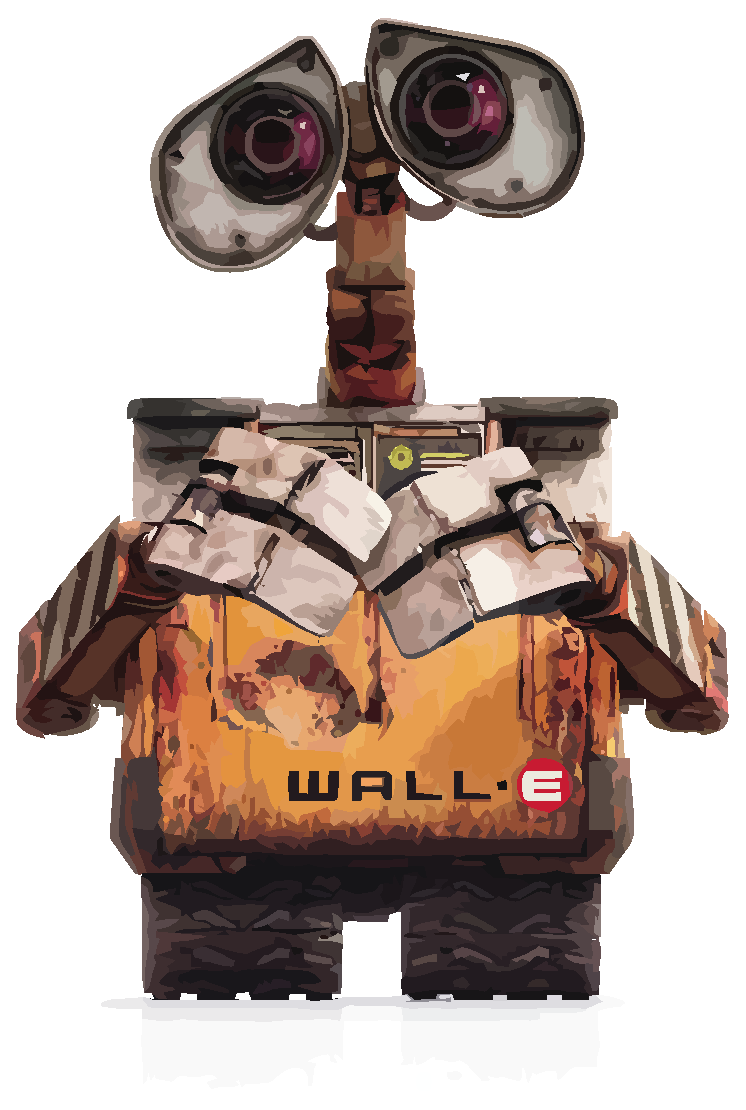
\includegraphics[width=\textwidth]{WallE}
      \caption{Wall-E}
      \label{fig:WallE}
    \end{subfigure}
    \begin{subfigure}[b]{0.3\textwidth}
      
\includegraphics[width=\textwidth]{minion}
      \caption{Minions}
      \label{fig:Minnion}
    \end{subfigure}
    \caption{Best Animations}
    \label{fig:animations}
  \end{figure}


\end{landscape}

%%!TEX root = ../thesis.tex
%*******************************************************************************
%****************************** Third Chapter **********************************
%*******************************************************************************
\chapter{My third chapter}

% **************************** Define Graphics Path **************************
\ifpdf
  \graphicspath{{Chapter/Chapter3/Figs/Raster/}{Chapter/Chapter3/Figs/PDF/}{Chapter/Chapter3/Figs/}}
\else
  \graphicspath{{Chapter/Chapter3/Figs/Vector/}{Chapter/Chapter3/Figs/}}
\fi

\section{First section of the third chapter}
And now I begin my third chapter here \dots

And now to cite some more people~\citet{Rea85,Ancey1996}

\subsection{First subsection in the first section}
\dots and some more

\subsection{Second subsection in the first section}
\dots and some more \dots

\subsubsection{First subsub section in the second subsection}
\dots and some more in the first subsub section otherwise it all looks the same
doesn't it? well we can add some text to it \dots

\subsection{Third subsection in the first section}
\dots and some more \dots

\subsubsection{First subsub section in the third subsection}
\dots and some more in the first subsub section otherwise it all looks the same
doesn't it? well we can add some text to it and some more and some more and
some more and some more and some more and some more and some more \dots

\subsubsection{Second subsub section in the third subsection}
\dots and some more in the first subsub section otherwise it all looks the same
doesn't it? well we can add some text to it \dots

\section{Second section of the third chapter}
and here I write more \dots

\section{The layout of formal tables}
This section has been modified from ``Publication quality tables in \LaTeX*''
by Simon Fear.

The layout of a table has been established over centuries of experience and
should only be altered in extraordinary circumstances.

When formatting a table, remember two simple guidelines at all times:

\begin{enumerate}
  \item Never, ever use vertical rules (lines).
  \item Never use double rules.
\end{enumerate}

These guidelines may seem extreme but I have
never found a good argument in favour of breaking them. For
example, if you feel that the information in the left half of
a table is so different from that on the right that it needs
to be separated by a vertical line, then you should use two
tables instead. Not everyone follows the second guideline:

There are three further guidelines worth mentioning here as they
are generally not known outside the circle of professional
typesetters and subeditors:

\begin{enumerate}\setcounter{enumi}{2}
  \item Put the units in the column heading (not in the body of
        the table).
  \item Always precede a decimal point by a digit; thus 0.1
          {\em not} just .1.
  \item Do not use `ditto' signs or any other such convention to
        repeat a previous value. In many circumstances a blank
        will serve just as well. If it won't, then repeat the value.
\end{enumerate}

A frequently seen mistake is to use `\textbackslash begin\{center\}' \dots `\textbackslash end\{center\}' inside a figure or table environment. This center environment can cause additional vertical space. If you want to avoid that just use `\textbackslash centering'


\begin{table}
  \caption{A badly formatted table}
  \centering
  \label{table:bad_table}
  \begin{tabular}{|l|c|c|c|c|}
    \hline
                       & \multicolumn{2}{c}{Species I} & \multicolumn{2}{c|}{Species II}                \\
    \hline
    Dental measurement & mean                          & SD                              & mean  & SD   \\ \hline
    \hline
    I1MD               & 6.23                          & 0.91                            & 5.2   & 0.7  \\
    \hline
    I1LL               & 7.48                          & 0.56                            & 8.7   & 0.71 \\
    \hline
    I2MD               & 3.99                          & 0.63                            & 4.22  & 0.54 \\
    \hline
    I2LL               & 6.81                          & 0.02                            & 6.66  & 0.01 \\
    \hline
    CMD                & 13.47                         & 0.09                            & 10.55 & 0.05 \\
    \hline
    CBL                & 11.88                         & 0.05                            & 13.11 & 0.04 \\
    \hline
  \end{tabular}
\end{table}

\begin{table}
  \caption{A nice looking table}
  \centering
  \label{table:nice_table}
  \begin{tabular}{l c c c c}
    \hline
    \multirow{2}{*}{Dental measurement} & \multicolumn{2}{c}{Species I} & \multicolumn{2}{c}{Species II}                \\
    \cline{2-5}
                                        & mean                          & SD                             & mean  & SD   \\
    \hline
    I1MD                                & 6.23                          & 0.91                           & 5.2   & 0.7  \\

    I1LL                                & 7.48                          & 0.56                           & 8.7   & 0.71 \\

    I2MD                                & 3.99                          & 0.63                           & 4.22  & 0.54 \\

    I2LL                                & 6.81                          & 0.02                           & 6.66  & 0.01 \\

    CMD                                 & 13.47                         & 0.09                           & 10.55 & 0.05 \\

    CBL                                 & 11.88                         & 0.05                           & 13.11 & 0.04 \\
    \hline
  \end{tabular}
\end{table}


\begin{table}
  \caption{Even better looking table using booktabs}
  \centering
  \label{table:good_table}
  \begin{tabular}{l c c c c}
    \toprule
    \multirow{2}{*}{Dental measurement} & \multicolumn{2}{c}{Species I} & \multicolumn{2}{c}{Species II}                \\
    \cmidrule{2-5}
                                        & mean                          & SD                             & mean  & SD   \\
    \midrule
    I1MD                                & 6.23                          & 0.91                           & 5.2   & 0.7  \\

    I1LL                                & 7.48                          & 0.56                           & 8.7   & 0.71 \\

    I2MD                                & 3.99                          & 0.63                           & 4.22  & 0.54 \\

    I2LL                                & 6.81                          & 0.02                           & 6.66  & 0.01 \\

    CMD                                 & 13.47                         & 0.09                           & 10.55 & 0.05 \\

    CBL                                 & 11.88                         & 0.05                           & 13.11 & 0.04 \\
    \bottomrule
  \end{tabular}
\end{table}



% ********************************** Back Matter *******************************
% Backmatter should be commented out, if you are using appendices after References
%\backmatter

% ********************************** Bibliography ******************************
\begin{spacing}{0.9}

  % To use the conventional natbib style referencing
  % Bibliography style previews: http://nodonn.tipido.net/bibstyle.php
  % Reference styles: http://sites.stat.psu.edu/~surajit/present/bib.htm

  \bibliographystyle{apalike}
  %\bibliographystyle{unsrt} % Use for unsorted references  
  %\bibliographystyle{plainnat} % use this to have URLs listed in References
  %\cleardoublepage
  \bibliography{References/references} % Path to your References.bib file


  % If you would like to use BibLaTeX for your references, pass `custombib' as
  % an option in the document class. The location of 'reference.bib' should be
  % specified in the preamble.tex file in the custombib section.
  % Comment out the lines related to natbib above and uncomment the following line.

  %\printbibliography[heading=bibintoc, title={References}]


\end{spacing}

% ********************************** Appendices ********************************

\begin{appendices} % Using appendices environment for more functunality

  \printnomenclature
  % \printnomenclature[space] space can be set as 2em between symbol and description
  %\printnomenclature[3em]
  \chapter{Abbreviations}

\begin{acronym}[AAPC]
	\acro{gt}[GT]{ground truth}
	\acro{ekf}[EKF]{extended Kalman filter}
	\acro{mlp}[MLP]{multi layer perceptron}
	\acro{ml}[ML]{machine leaning}
	\acro{cnn}[CNN]{convolutional neural network}
	\acro{tsp}[TSP]{travelling salesman problem}
	\acro{slam}[SLAM]{simultaneous localization and mapping}
	\acro{fsd}[FSD]{Formula Student Driverless}
	\acro{ros}[ROS]{Robot Operation System}
	\acro{mppi}[MPPI]{model predictive path integral}
	\acro{relu}[ReLU]{Rectified Linear Unit}
	\acro{nn}[NN]{neural network}
	\acro{imu}[IMU]{inertial measurement unit}

\end{acronym}
  %!TEX root = ../thesis.tex
% ******************************* TrackVisualizerJS Documentation ****************************
\chapter{TrackVisualizerJS Documentation}

\end{appendices}

% *************************************** Index ********************************
\printthesisindex % If index is present

\end{document}
